\documentclass[final]{beamer}
\usepackage[T1]{fontenc}
\usepackage[utf8]{inputenc}
\usepackage{lmodern}
\usepackage{amsmath,amssymb}
\usepackage{graphicx}
\usepackage{ragged2e}
\usepackage{array}
\usepackage{booktabs}
\usepackage[table]{xcolor}
\usepackage[size=custom,width=185,height=90,scale=1.40]{beamerposter}

% This poster intentionally uses only scientific figures included in the PFF paper.
\graphicspath{{figures/}{logos/}}

\definecolor{PFFGreen}{RGB}{77,155,77}
\definecolor{PFFGreenDark}{RGB}{35,92,61}
\definecolor{PFFMint}{RGB}{231,245,232}
\definecolor{PFFText}{RGB}{35,42,48}
\definecolor{PFFMuted}{RGB}{92,103,111}
\definecolor{PFFBlue}{RGB}{49,139,181}
\definecolor{PFFOrange}{RGB}{220,105,38}
\definecolor{PFFRule}{RGB}{204,221,208}

\setbeamercolor{normal text}{fg=PFFText,bg=white}
\setbeamercolor{block title}{fg=white,bg=PFFGreenDark}
\setbeamercolor{block body}{fg=PFFText,bg=white}
\setbeamercolor{itemize item}{fg=PFFGreenDark}
\setbeamercolor{itemize subitem}{fg=PFFGreenDark}
\setbeamercolor{pff highlight}{fg=PFFGreenDark,bg=PFFMint}
\setbeamercolor{pff mode}{fg=PFFText,bg=PFFMint}

\setbeamerfont{title}{series=\bfseries,size=\fontsize{92}{100}}
\setbeamerfont{author}{size=\fontsize{32}{37}}
\setbeamerfont{institute}{size=\fontsize{25}{30}}
\setbeamerfont{block title}{series=\bfseries,size=\fontsize{42}{47}}
\setbeamerfont{block body}{size=\fontsize{29}{33}}
\setbeamerfont{caption}{size=\fontsize{20}{23}}

\setbeamertemplate{navigation symbols}{}
\setbeamertemplate{itemize item}{\raisebox{0.12em}{\tiny$\blacktriangleright$}}
\setbeamertemplate{itemize subitem}{\raisebox{0.12em}{\tiny$\blacktriangleright$}}
\setbeamertemplate{block begin}{%
  \vspace{0.12cm}
  \begin{center}
  \begin{beamercolorbox}[wd=0.97\linewidth,ht=1.38cm,dp=0.20cm,leftskip=0.38cm,rightskip=0.35cm]{block title}
    \usebeamerfont{block title}\strut\insertblocktitle\strut
  \end{beamercolorbox}
  \end{center}
  \vspace{0.10cm}
  \begin{beamercolorbox}[wd=\linewidth,sep=0.10cm]{block body}
    \usebeamerfont{block body}
}
\setbeamertemplate{block end}{%
  \end{beamercolorbox}
  \vspace{0.08cm}
}
\setlength{\leftmargini}{1.05em}
\setlength{\leftmarginii}{0.85em}
\setlength{\columnsep}{1.7cm}
\emergencystretch=3em

\pdfstringdefDisableCommands{%
  \def\textsuperscript#1{ (#1)}%
  \def\and{, }%
}

\hypersetup{
  pdftitle={Prior-Fitted Functional Flows: In-Context Generative Models for Pharmacokinetics},
  pdfauthor={Cesar Ojeda et al.}
}

\title{Prior-Fitted Functional Flows:\\[-0.08em]
In-Context Generative Models for Pharmacokinetics}
\author{C\'esar Ojeda\textsuperscript{1} \and Niklas Hartung\textsuperscript{1} \and Wilhelm Huisinga\textsuperscript{1} \and Tim Jahn\textsuperscript{2} \and Purity Kamene Kavwele\textsuperscript{1} \and Marian Klose\textsuperscript{3} \\
Piyush Kumar\textsuperscript{1} \and Rams\'es J. S\'anchez\textsuperscript{4} \and Darius A. Faroughy\textsuperscript{5}}
\institute{\textsuperscript{1}University of Potsdam \quad
\textsuperscript{2}Technical University Berlin \quad
\textsuperscript{3}Freie Universit\"at Berlin \quad
\textsuperscript{4}Lamarr Institute \& University of Bonn \quad
\textsuperscript{5}NHETC, Rutgers University, USA}

\newcommand{\PFF}{\textbf{PFF}}
\newcommand{\subhead}[1]{\vspace{0.16em}{\color{PFFGreenDark}\bfseries #1}\par\vspace{0.10em}}
\newcommand{\emline}[1]{{\color{PFFGreenDark}\bfseries #1}}
\newcommand{\logoimg}[1]{\includegraphics[height=5.6cm,keepaspectratio]{#1}}
\newcommand{\takeaway}[1]{%
  \vspace{0.18em}
  \begin{beamercolorbox}[wd=\linewidth,rounded=true,sep=0.65em]{pff highlight}
    \textbf{Takeaway.} #1
  \end{beamercolorbox}
}
\newcommand{\modebox}[2]{%
  \begin{beamercolorbox}[wd=\linewidth,rounded=true,sep=0.55em]{pff mode}
    {\color{PFFGreenDark}\bfseries #1}\par #2
  \end{beamercolorbox}
}

\begin{document}
\begin{frame}[t]

% Header ----------------------------------------------------------------------
\begin{beamercolorbox}[wd=\paperwidth,sep=1.15cm,leftskip=3.5cm,rightskip=2.0cm]{block body}
  \begin{columns}[T,totalwidth=\textwidth]
    \begin{column}{0.67\textwidth}
      \hspace*{0.6cm}\parbox[t]{0.96\linewidth}{%
        {\usebeamerfont{title}\color{PFFText}\inserttitle\par}
        \vspace{0.42cm}
        {\usebeamerfont{author}\color{PFFText}\insertauthor\par}
        \vspace{0.22cm}
        {\usebeamerfont{institute}\color{PFFMuted}\insertinstitute\par}
        \vspace{0.18cm}
        {\usebeamerfont{institute}\color{PFFMuted}\textit{Contact:} ojedamarin@uni-potsdam.de
        \quad \textit{Code, model, data:} github.com/cesarali/pff}
      }
    \end{column}
    \begin{column}{0.27\textwidth}
      \centering
      \makebox[\linewidth][c]{%
        \logoimg{tu-potsdam.pdf}\hspace{1.7cm}%
        \logoimg{lamarr-logo-2023.png}\hspace{1.7cm}%
        \logoimg{uni_bonn.png}\hspace{1.7cm}%
        \logoimg{SFB1294.png}%
      }
    \end{column}
  \end{columns}
\end{beamercolorbox}

\vspace{-0.45cm}

\begin{columns}[T,totalwidth=\textwidth]

% Column 1 --------------------------------------------------------------------
\begin{column}{0.285\textwidth}

\begin{block}{Problem \& Core Idea}
\justifying
\small

\subhead{Sparse cohorts, continuous trajectories}
A pharmacokinetic study is a set of sparse, noisy, and irregularly sampled
concentration--time series from a small cohort,
\(
\mathcal S=\{\mathcal D^1,\ldots,\mathcal D^I\}.
\)
For a new individual, we want a \emline{distribution over plausible concentration functions}---not just one point estimate---conditioned on the cohort and, optionally, a few early observations.

\vspace{0.20em}
\begin{figure}
  \centering
  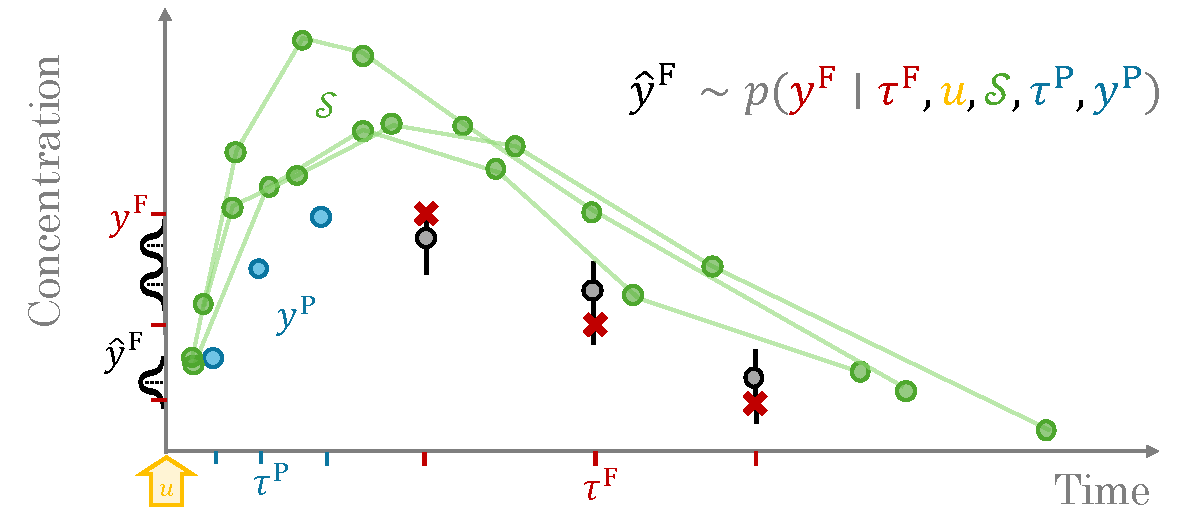
\includegraphics[width=0.84\linewidth]{NotationIllustration_FlowMatching.pdf}
  \vspace{-0.45em}
  \caption{Study context $\mathcal S$ (green) and a patient's observed prefix (blue) define a distribution over future concentration values (gray/red).}
\end{figure}
\vspace{-0.42em}

\subhead{Why prior fitting?}
Classical nonlinear mixed-effects models require study-specific design, optimization, and diagnostics. High-capacity neural models are difficult to fit reliably to each small trial. \PFF{} shifts that cost to a single pretraining stage:
\begin{itemize}
  \setlength\itemsep{0.10em}
  \item pretrain on diverse, mechanistically simulated PK studies;
  \item learn reusable inference directly in function space;
  \item deploy zero-shot to a new compound without fine-tuning.
\end{itemize}

\takeaway{One pretrained conditional flow supports both virtual-cohort generation and patient-level forecasting.}
\end{block}

\begin{block}{Physiologically Calibrated Prior}
\justifying
\small

The simulator combines compartmental ODE systems with stochastic, time-varying parameters, diverse dosing routes and structures, and irregular sampling schedules. Its priors are calibrated against an open-access corpus of PK parameters mined from clinical bioequivalence studies.

\vspace{0.20em}
\begin{figure}
  \centering
  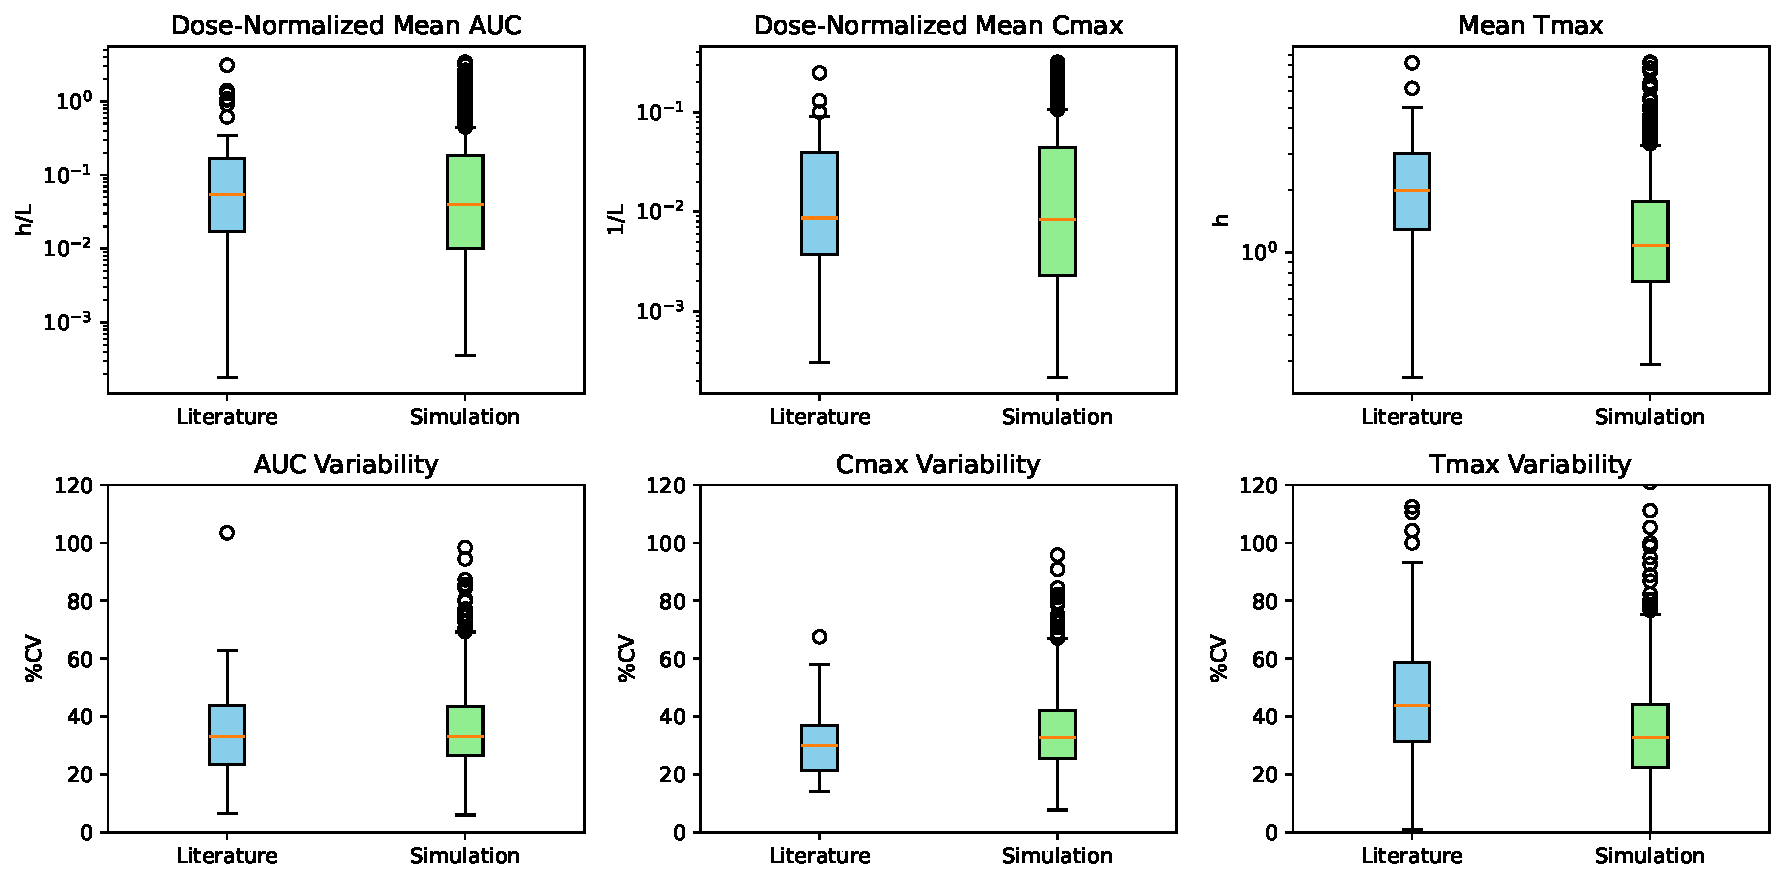
\includegraphics[width=0.78\linewidth]{pk-metrics-literature-vs-simulation.pdf}
  \vspace{-0.40em}
  \caption{Literature (blue) and simulation (green) distributions for exposure, peak concentration, peak time, and their inter-individual variability.}
\end{figure}
\vspace{-0.40em}

{\footnotesize\color{PFFGreenDark}\textbf{Result.} Literature calibration anchors the synthetic pretraining distribution to realistic scales and inter-individual variability.}
\end{block}

\end{column}

% Column 2 --------------------------------------------------------------------
\begin{column}{0.365\textwidth}

\begin{block}{Prior-Fitted Functional Flow}
\justifying
\small

\subhead{Conditional transport in function space}
\PFF{} learns a time-dependent neural-operator vector field that transports a tractable Gaussian-process (GP) reference measure into the conditional distribution of concentration functions induced by the PK simulator.

\vspace{0.16em}
\begin{columns}[T,totalwidth=\linewidth]
  \begin{column}{0.48\linewidth}
    \modebox{Population synthesis ($p=0$)}{Start from a GP prior over a full trajectory and transport it using study-level context $\mathcal S$.}
  \end{column}
  \begin{column}{0.48\linewidth}
    \modebox{Forecasting ($p>0$)}{Start from a GP posterior given the observed prefix; transport only the unobserved continuation.}
  \end{column}
\end{columns}

\vspace{0.20em}
The unified reference measure is
\[
\eta_{\mathrm F}(\cdot\mid o,p)=
\begin{cases}
\mathrm{GP}_{\mathcal T_{\mathrm F}}(\cdot\mid \mathbf u,\mathbf y_{\mathrm P}), & p>0,\\[2pt]
\mathrm{GP}_{\mathcal T_{\mathrm F}}(\cdot), & p=0.
\end{cases}
\]
For a sampled split, define
\(
\mathbf z_0=(\mathbf y_{\mathrm P},\mathbf x_{\mathrm F})
\)
and
\(
\mathbf z_1=(\mathbf y_{\mathrm P},\mathbf y_{\mathrm F}).
\)
The Gaussian conditional path and masked flow-matching objective are
\[
\mathbf z_t\sim
\mathcal N\!\left(t\mathbf z_1+(1-t)\mathbf z_0,\sigma_{\min}^2I\right),
\]
\vspace{-0.35em}
\[
\mathcal L(\theta)=
\mathbb E\!\left[
\left\|\mathbf M_p\odot v_t^\theta(\mathbf z_t,c)
-(\mathbf y_{\mathrm F}-\mathbf x_{\mathrm F})\right\|^2
\right].
\]
The prefix-dependent mask $\mathbf M_p$ keeps the observed past fixed while the learned vector field transports uncertainty in the future.

\vspace{0.16em}
\begin{figure}
  \centering
  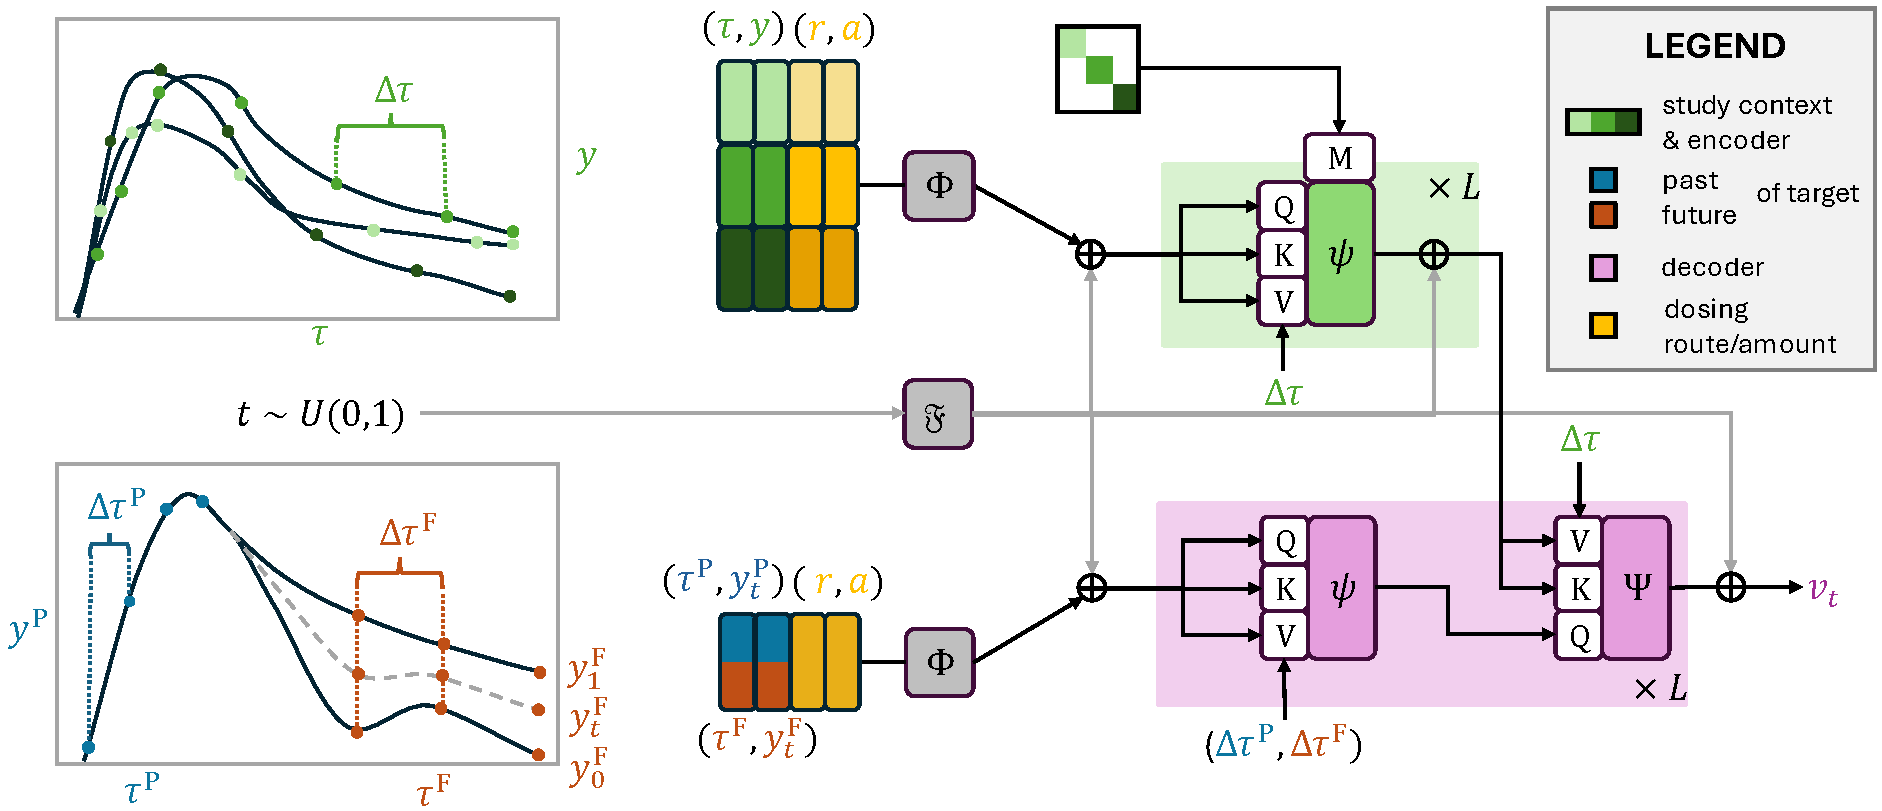
\includegraphics[width=0.98\linewidth]{NetworkArchitectureSketch-FlowMatching.pdf}
  \vspace{-0.38em}
  \caption{Operator encoder--decoder vector field. The context encoder summarizes individuals without mixing subjects; the target decoder combines the interpolated trajectory, dosing, flow time, and study context.}
\end{figure}
\vspace{-0.40em}

\subhead{Continuum-attention neural operator}
Observation grids differ across subjects and are not aligned. Encoder self-attention and decoder self-/cross-attention therefore use continuum-operator attention with trapezoidal quadrature corrections. This makes the learned vector field resolution- and grid-aware while retaining a transformer encoder--decoder structure.

\takeaway{GP posterior initialization enforces prefix consistency; triangular transport and continuum attention generate coherent futures on irregular time grids.}
\end{block}

\end{column}

% Column 3 --------------------------------------------------------------------
\begin{column}{0.315\textwidth}

\begin{block}{Zero-Shot Individual Forecasting}
\small
\begin{figure}
  \centering
  \begin{minipage}[b]{0.315\linewidth}
    \centering
    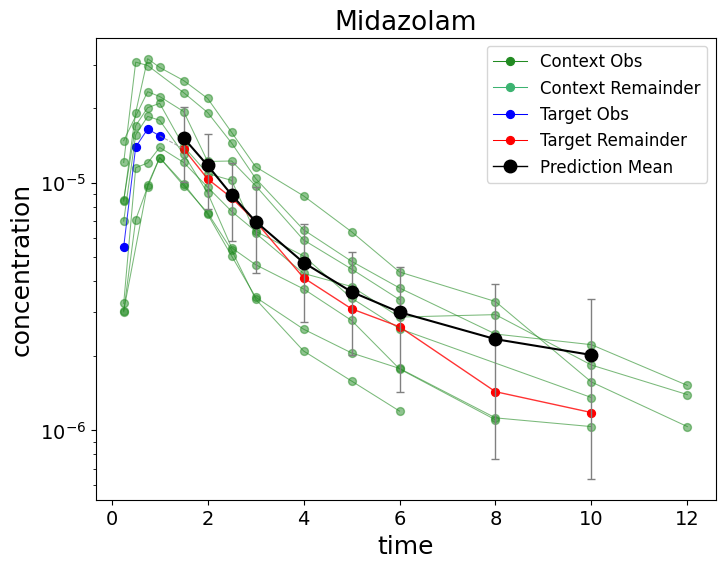
\includegraphics[width=0.68\linewidth]{midazolam_prediction.png}\\[-0.20em]
    {\footnotesize Midazolam}
  \end{minipage}\hfill
  \begin{minipage}[b]{0.315\linewidth}
    \centering
    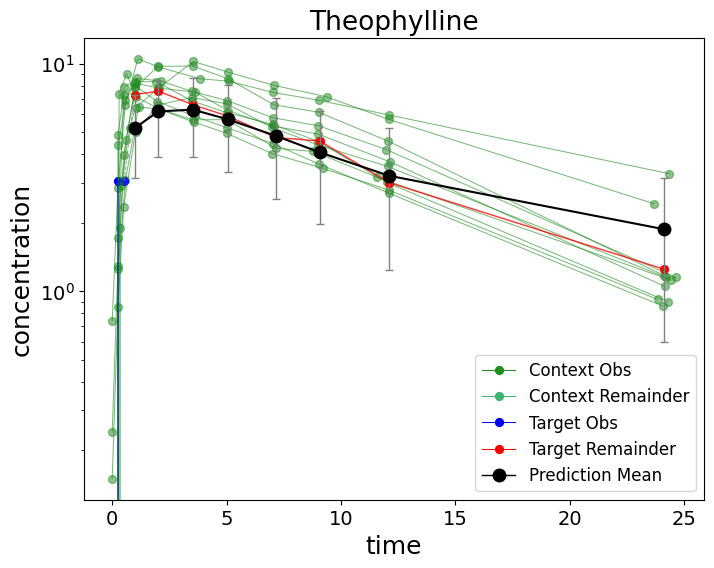
\includegraphics[width=0.68\linewidth]{theophylline_prediction.png}\\[-0.20em]
    {\footnotesize Theophylline}
  \end{minipage}\hfill
  \begin{minipage}[b]{0.315\linewidth}
    \centering
    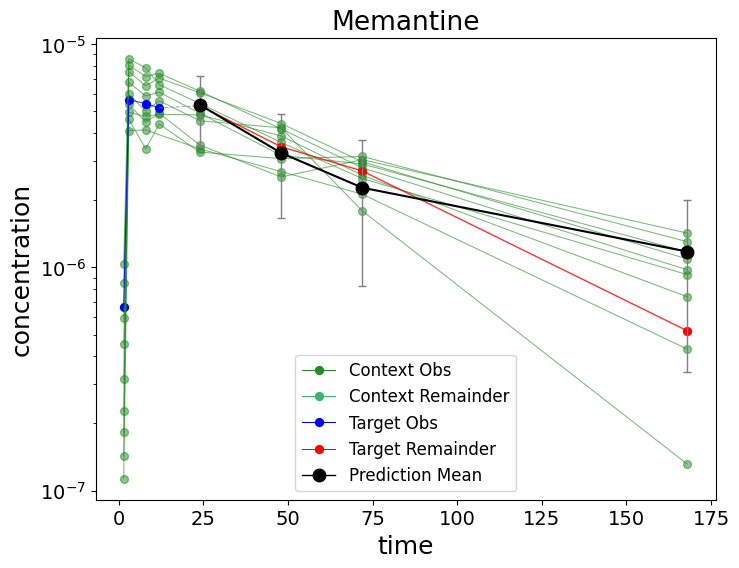
\includegraphics[width=0.68\linewidth]{memantine_prediction.png}\\[-0.20em]
    {\footnotesize Memantine}
  \end{minipage}
  \vspace{-0.35em}
  \caption{Conditioned on the cohort (green) and four early patient measurements (blue), PFF samples future trajectories (red); black denotes the predictive mean.}
\end{figure}
\end{block}

\begin{block}{Selected Forecasting Accuracy (Log-RMSE)}
\small
\centering
{\fontsize{14}{17}\selectfont
\renewcommand{\arraystretch}{0.98}
\setlength{\tabcolsep}{4pt}
\resizebox{0.98\linewidth}{!}{%
\begin{tabular}{lccccc}
\toprule
\textbf{Compound} & \textbf{NLME} & \textbf{Transf.} & \textbf{NODE} & \textbf{AICMET} & \textbf{PFF} \\
\midrule
caffeine & $0.294$ & $0.451$ & $0.432$ & $0.399$ & $\mathbf{0.174}$ \\
indometacin & $0.582$ & $0.429$ & $0.350$ & $0.536$ & $\mathbf{0.245}$ \\
omeprazole & $1.300$ & $0.842$ & $1.003$ & $0.936$ & $\mathbf{0.593}$ \\
theophylline & $0.732$ & $0.356$ & $0.327$ & $0.274$ & $\mathbf{0.184}$ \\
tolbutamide & $0.723$ & $0.678$ & $0.578$ & $0.517$ & $\mathbf{0.421}$ \\
1-OH-midazolam & -- & $0.567$ & $0.737$ & $0.491$ & $\mathbf{0.422}$ \\
\bottomrule
\end{tabular}}
}
\vspace{0.12em}

{\footnotesize Mean leave-one-individual-out log-RMSE. The table shows representative compounds from the paper on which PFF is best. Evaluation uses the first four observations as individual context.}
\end{block}

\begin{block}{Population Synthesis \& Ablations}
\small
\begin{figure}
  \centering
  \begin{minipage}[b]{0.48\linewidth}
    \centering
    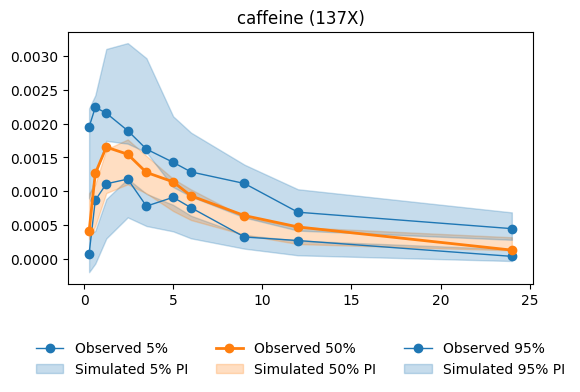
\includegraphics[width=0.66\linewidth]{caffeine_vpc.png}\\[-0.20em]
    {\footnotesize Caffeine}
  \end{minipage}\hfill
  \begin{minipage}[b]{0.48\linewidth}
    \centering
    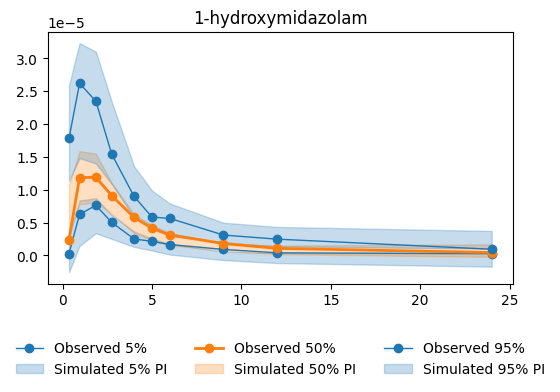
\includegraphics[width=0.66\linewidth]{1_hydroxymidazolam_vpc.png}\\[-0.20em]
    {\footnotesize 1-hydroxy-midazolam}
  \end{minipage}
  \vspace{-0.40em}
  \caption{Visual predictive checks: observed concentration summaries versus simulation-derived prediction intervals.}
\end{figure}
\vspace{-0.45em}

{\fontsize{13}{16}\selectfont
\centering
\renewcommand{\arraystretch}{0.94}
\setlength{\tabcolsep}{7pt}
\begin{tabular}{lcc}
\toprule
\textbf{Synthetic evaluation} & \textbf{AUC}$\downarrow 0.5$ & \textbf{MMD}$\downarrow 0$ \\
\midrule
AICMET & $0.54\pm0.01$ & $0.002\pm0.001$ \\
PFF & $\mathbf{0.52\pm0.01}$ & $\mathbf{0.001\pm0.001}$ \\
PFF--standard attention & $0.61\pm0.03$ & $0.004\pm0.004$ \\
PFF--white noise & $0.59\pm0.05$ & $0.004\pm0.001$ \\
\bottomrule
\end{tabular}
}

\vspace{0.14em}
{\footnotesize Generated trajectories are harder to distinguish from references than AICMET samples. Removing either the GP posterior or continuum attention degrades fidelity. Sampling 100 virtual individuals takes about $3.5$\,s on one A100 GPU.}

{\footnotesize\color{PFFGreenDark}\textbf{Result.} PFF combines accurate forecasting with faithful zero-shot cohort synthesis; both the reference measure and operator architecture matter.}
\end{block}

\end{column}
\end{columns}

\end{frame}
\end{document}
